\section{Arquitectura del sistema}\label{section:arquitecturaSistema}
La estructura principal del sistema es una aplicación en la nube denominada
\emph{Nube de Conductores}. Se encarga de hacer llegar los mensajes procedentes
de los ciclistas a los vehículos a motor, y los mensajes enviados por los vehículos
a motor a los ciclistas. Además, filtra los mensajes que han sido mal formados,
monitoriza las posiciones de todos los vehículos en la carretera y es capaz de
predecir cuándo se puede dar la posibilidad de que haya un choque entre dos vehículos;
en cuyo caso avisa a los conductores de esta posibilidad.

Los vehículos a motor se mantienen mandando continuamente beacons a través de un
\gls{obu}. Para enviar los mensajes emplean el canal broadcast de la red 802.11p.
En estos mensajes anuncian al resto de vehículos su posición, velocidad y dirección
hacia la que circulan. No se comunican directamente con la \emph{Nube de Conductores},
sino que los mensajes enviados son escuchados por unidades desplegadas en carretera
llamada \gls{rsu}.

La \gls{rsu} recibe los mensajes que envían los vehículos y retransmiten esta
información a la \emph{Nube de Conductores}. Así mismo, retransmiten los mensajes
que reciben de la nube a los vehículos en carretera; a excepción de que el
destinatario sea la propia \gls{rsu}.

Por otro lado, los ciclistas envían información a la \emph{Nube de Conductores} a
través de redes móviles; dependiendo de la disponibilidad, 3G o 4G. Éstos también
pueden agruparse empleando la red \emph{Wi-Fi 802.11}, mediante la creación de un
HUB para dispositivos móviles en el cual se envían notificaciones sobre los eventos
que aparezcan.

En la figura \ref{fig:ArquitecturaSistema} se puede observar de qué elementos está
compuesto el sistema y cómo se comunican entre ellos. Como puede apreciarse, hay
diferentes tecnologías de comunicación y desarrollo en cada una de las plataformas,
por lo que uno de los requisitos es que la solución desarrollada sea flexible a los
cambios de tecnología tanto comunicación como desarrollo.

\begin{figure}[H]
	\begin{center}
		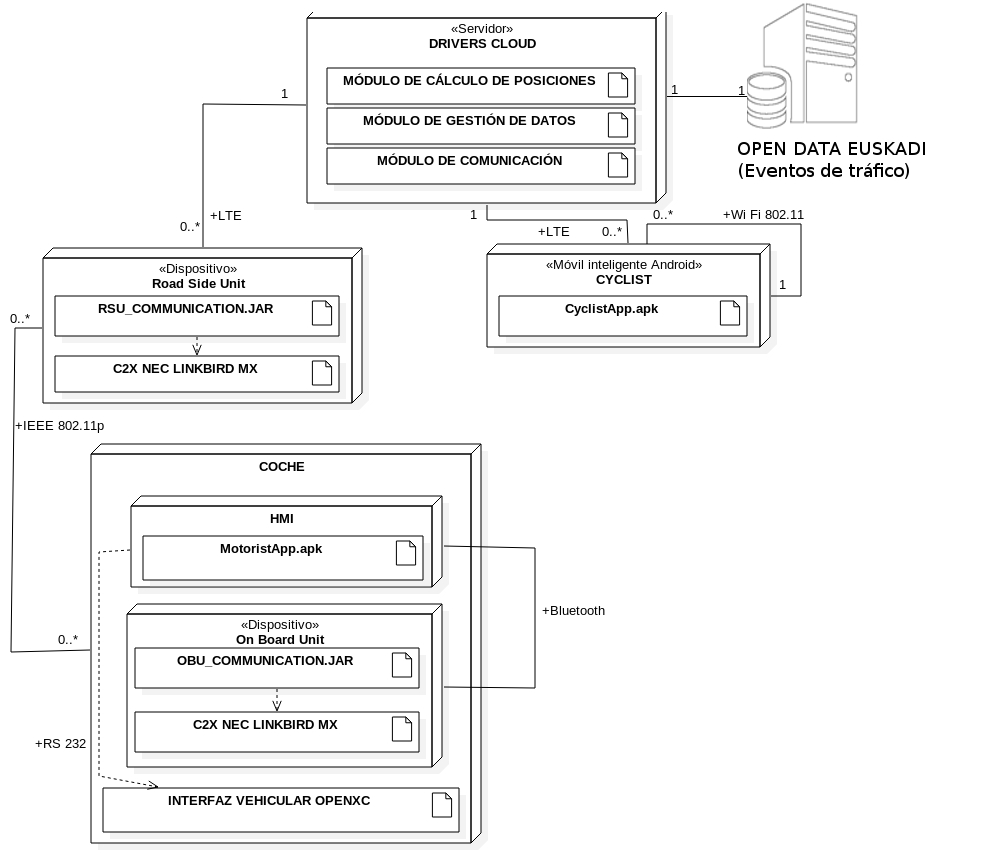
\includegraphics[scale=0.4]{arquitectura_global}
		\caption{Arquitectura del sistema}
		\label{fig:ArquitecturaSistema}
	 \end{center}
\end{figure}
